\begin{figure}[H]
\centering
\includegraphics[page=6,width=0.48\textwidth]{\FCNCFigures/tthML/showFake/faketau/prefit/NOMINAL/reg1l1tau1b1j_ss_vetobtagwp70_highmet/tau_pt_0.pdf}
\includegraphics[page=6,width=0.48\textwidth]{\FCNCFigures/tthML/showFake/faketau/prefit/NOMINAL/reg1l1tau1b2j_ss_vetobtagwp70_highmet/tau_pt_0.pdf}
\includegraphics[page=6,width=0.48\textwidth]{\FCNCFigures/tthML/showFake/faketau/prefit/NOMINAL/reg1l1tau1b2j_os_vetobtagwp70_highmet/tau_pt_0.pdf}
\includegraphics[page=6,width=0.48\textwidth]{\FCNCFigures/tthML/showFake/faketau/prefit/NOMINAL/reg1l1tau1b3j_os_vetobtagwp70_highmet/tau_pt_0.pdf}
\includegraphics[page=6,width=0.48\textwidth]{\FCNCFigures/tthML/showFake/faketau/prefit/NOMINAL/reg1l2tau1bnj_os/tau_pt_0.pdf}

\caption{轻子道信号区中$\tauhad$的$\pt$谱,图中将Fake tau的来源进行分类,其中的Fake tau本底包含所有的样本。}
\label{fig:wjet_pt}
\end{figure}
